\documentclass{standalone}

% Required package
\usepackage{tikz}

\begin{document}
	
	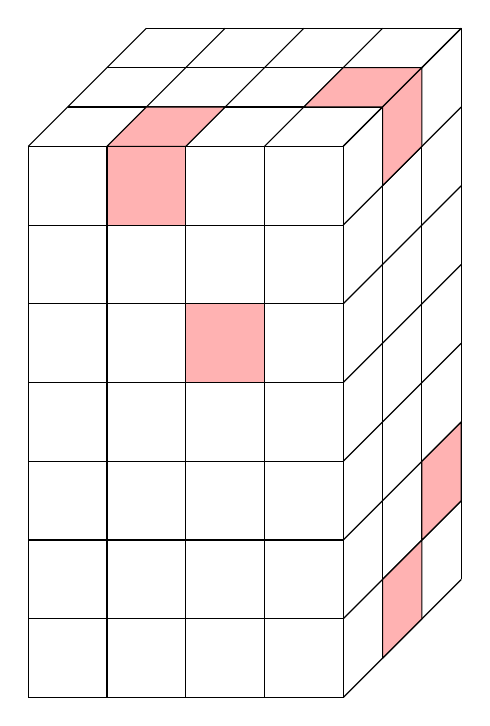
\begin{tikzpicture}
		
		% THE 3D STRUCTURE
		\draw[-] (-2,0) -- (2,0);
		\draw[-] (-2,-7) -- (-2,0);
		\draw[-] (-2,-7) -- (2,-7);
		\draw[-] (2,-7) -- (2,0);
		\draw[-] (-2,0) -- (-0.5,1.5);
		\draw[-] (2,0) -- (3.5,1.5);
		\draw[-] (-0.5,1.5) -- (3.5,1.5);
		\draw[-] (2,-7) -- (3.5,-5.5);
		\draw[-] (3.5,1.5) -- (3.5,-5.5);
		%
		% THE ROWS AND COLUMNS
		% FRONT SIDE
		% ROWS
		\draw[-] (-2,-1) -- (2,-1);
		\draw[-] (-2,-2) -- (2,-2);
		\draw[-] (-2,-3) -- (2,-3);
		\draw[-] (-2,-4) -- (2,-4);
		\draw[-] (-2,-5) -- (2,-5);
		\draw[-] (-2,-6) -- (2,-6);
		% COLUMNS
		\draw[-] (-1,0) -- (-1,-7);
		\draw[-] (0,0) -- (0,-7);
		\draw[-] (1,0) -- (1,-7);
		%
		% UP SIDE
		% COLUMNS
		\draw[-] (-1,0) -- (0.5,1.5);
		\draw[-] (0,0) -- (1.5,1.5);
		\draw[-] (1,0) -- (2.5,1.5);
		% ROWS
		\draw[-] (-1.5,0.5) -- (2.5,0.5);
		\draw[-] (-1,1) -- (3,1);
		%
		% RIGHT SIDE
		% ROWS
		\draw[-] (2,0) -- (3.5,1.5);
		\draw[-] (2,-1) -- (3.5,0.5);
		\draw[-] (2,-2) -- (3.5,-0.5);
		\draw[-] (2,-3) -- (3.5,-1.5);
		\draw[-] (2,-4) -- (3.5,-2.5);
		\draw[-] (2,-5) -- (3.5,-3.5);
		\draw[-] (2,-6) -- (3.5,-4.5);
		% COLUMNS
		\draw[-] (2.5,0.5) -- (2.5,-6.5);
		\draw[-] (3,1) -- (3,-6);
		%
		%
		% THE FILLS!
		% FRONT FILL
		\path [fill=red!30, draw=black,]
		(-1,0) -- (0,0) -- (0,-1) -- (-1,-1) -- (-1,0);
		\path [fill=red!30, draw=black,]
		(0,-2) -- (1,-2) -- (1,-3) -- (0,-3) -- (0,-2);
		% RIGHT FILL
		\path [fill=red!30, draw=black,]
		(2.5,-6.5) -- (3,-6) -- (3,-5) -- (2.5,-5.5) -- (2.5,-6.5);
		\path [fill=red!30, draw=black,]
		(3,-5) -- (3.5,-4.5) -- (3.5,-3.5) -- (3,-4) -- (3,-5);
		% UP FILL
		\path [fill=red!30, draw=black,]
		(-1,0) -- (0,0) -- (0.5,0.5) -- (-0.5,0.5) -- (-1,0);
		\path [fill=red!30, draw=black,]
		(1.5,0.5) -- (2.5,0.5) -- (3,1) -- (2,1) -- (1.5,0.5);
		\path [fill=red!30, draw=black,]
		(2.5,0.5) -- (3,1) -- (3,0) -- (2.5,-0.5) -- (2.5,0.5);
	\end{tikzpicture}
	
\end{document}